
\section{Metodologia}

A metodologia adotada neste trabalho foi estruturada para permitir uma análise comparativa rigorosa entre diferentes algoritmos de controle cooperativo de formação de VANTs (Veículos Aéreos Não Tripulados). A abordagem é experimental, quantitativa e fundamentada em simulações computacionais, de modo a garantir reprodutibilidade, isolamento de variáveis e segurança no estudo de comportamento coletivo. O processo foi dividido em quatro etapas principais: (i) definição dos algoritmos e cenários; (ii) implementação dos modelos de controle; (iii) execução das simulações; e (iv) análise dos resultados.

Inicialmente, serão selecionados os algoritmos amplamente utilizados em controle cooperativo de formação. Entre eles, temos:

\begin{itemize}
    \item \textbf{Leader–Follower}: estrutura hierárquica em que um agente líder define a trajetória e os seguidores ajustam suas posições relativas;
    \item \textbf{Consensus-Based}: cada agente atualiza seu estado com base nos vizinhos, buscando convergência coletiva;
    \item \textbf{Behavior-Based}: comportamentos individuais (coesão, separação, alinhamento) geram padrões emergentes;
    \item \textbf{Virtual Structure}: a formação é tratada como uma estrutura rígida virtual, com posições relativas predefinidas;
    \item \textbf{Artificial Potential Fields (APF)}: o movimento decorre de forças atrativas e repulsivas que moldam o posicionamento desejado.
\end{itemize}

Com o objetivo de investigar potenciais melhorias no desempenho, também serão consideradas combinações híbridas de algoritmos, explorando complementaridades entre abordagens — por exemplo, a combinação entre \textit{Consensus-Based} e \textit{APF} para simultaneamente manter coesão e evitar colisões.

As simulações serão realizadas utilizando o simulador \textit{Gazebo}, integrado ao middleware \textit{ROS2} e ao firmware PX4 Autopilot em modo SITL (\textit{Software-In-The-Loop}), conforme ilustrado na Figura~\ref{fig:Arquitetura de simulação}. Essa escolha se justifica por três razões principais: (i) o \textit{Gazebo} fornece um ambiente tridimensional realista com motores de física robustos, permitindo simulação de dinâmicas e colisões com alta fidelidade; (ii) o \textit{ROS2} possibilita arquitetura modular, comunicação determinística e suporte nativo a sistemas distribuídos, características essenciais para experimentos com múltiplos agentes; e (iii) o PX4 SITL permite emular o comportamento do autopiloto real, utilizando o protocolo MAVLink para comandar cada VANT, o que preserva a compatibilidade com sistemas embarcados reais e facilita a futura transição para testes em campo. As implementações dos controladores serão desenvolvidas em \textit{Python}, com o uso de \textit{NumPy} para cálculos numéricos e \textit{Matplotlib} para análise gráfica.

\begin{figure*}[ht]
    \centering
    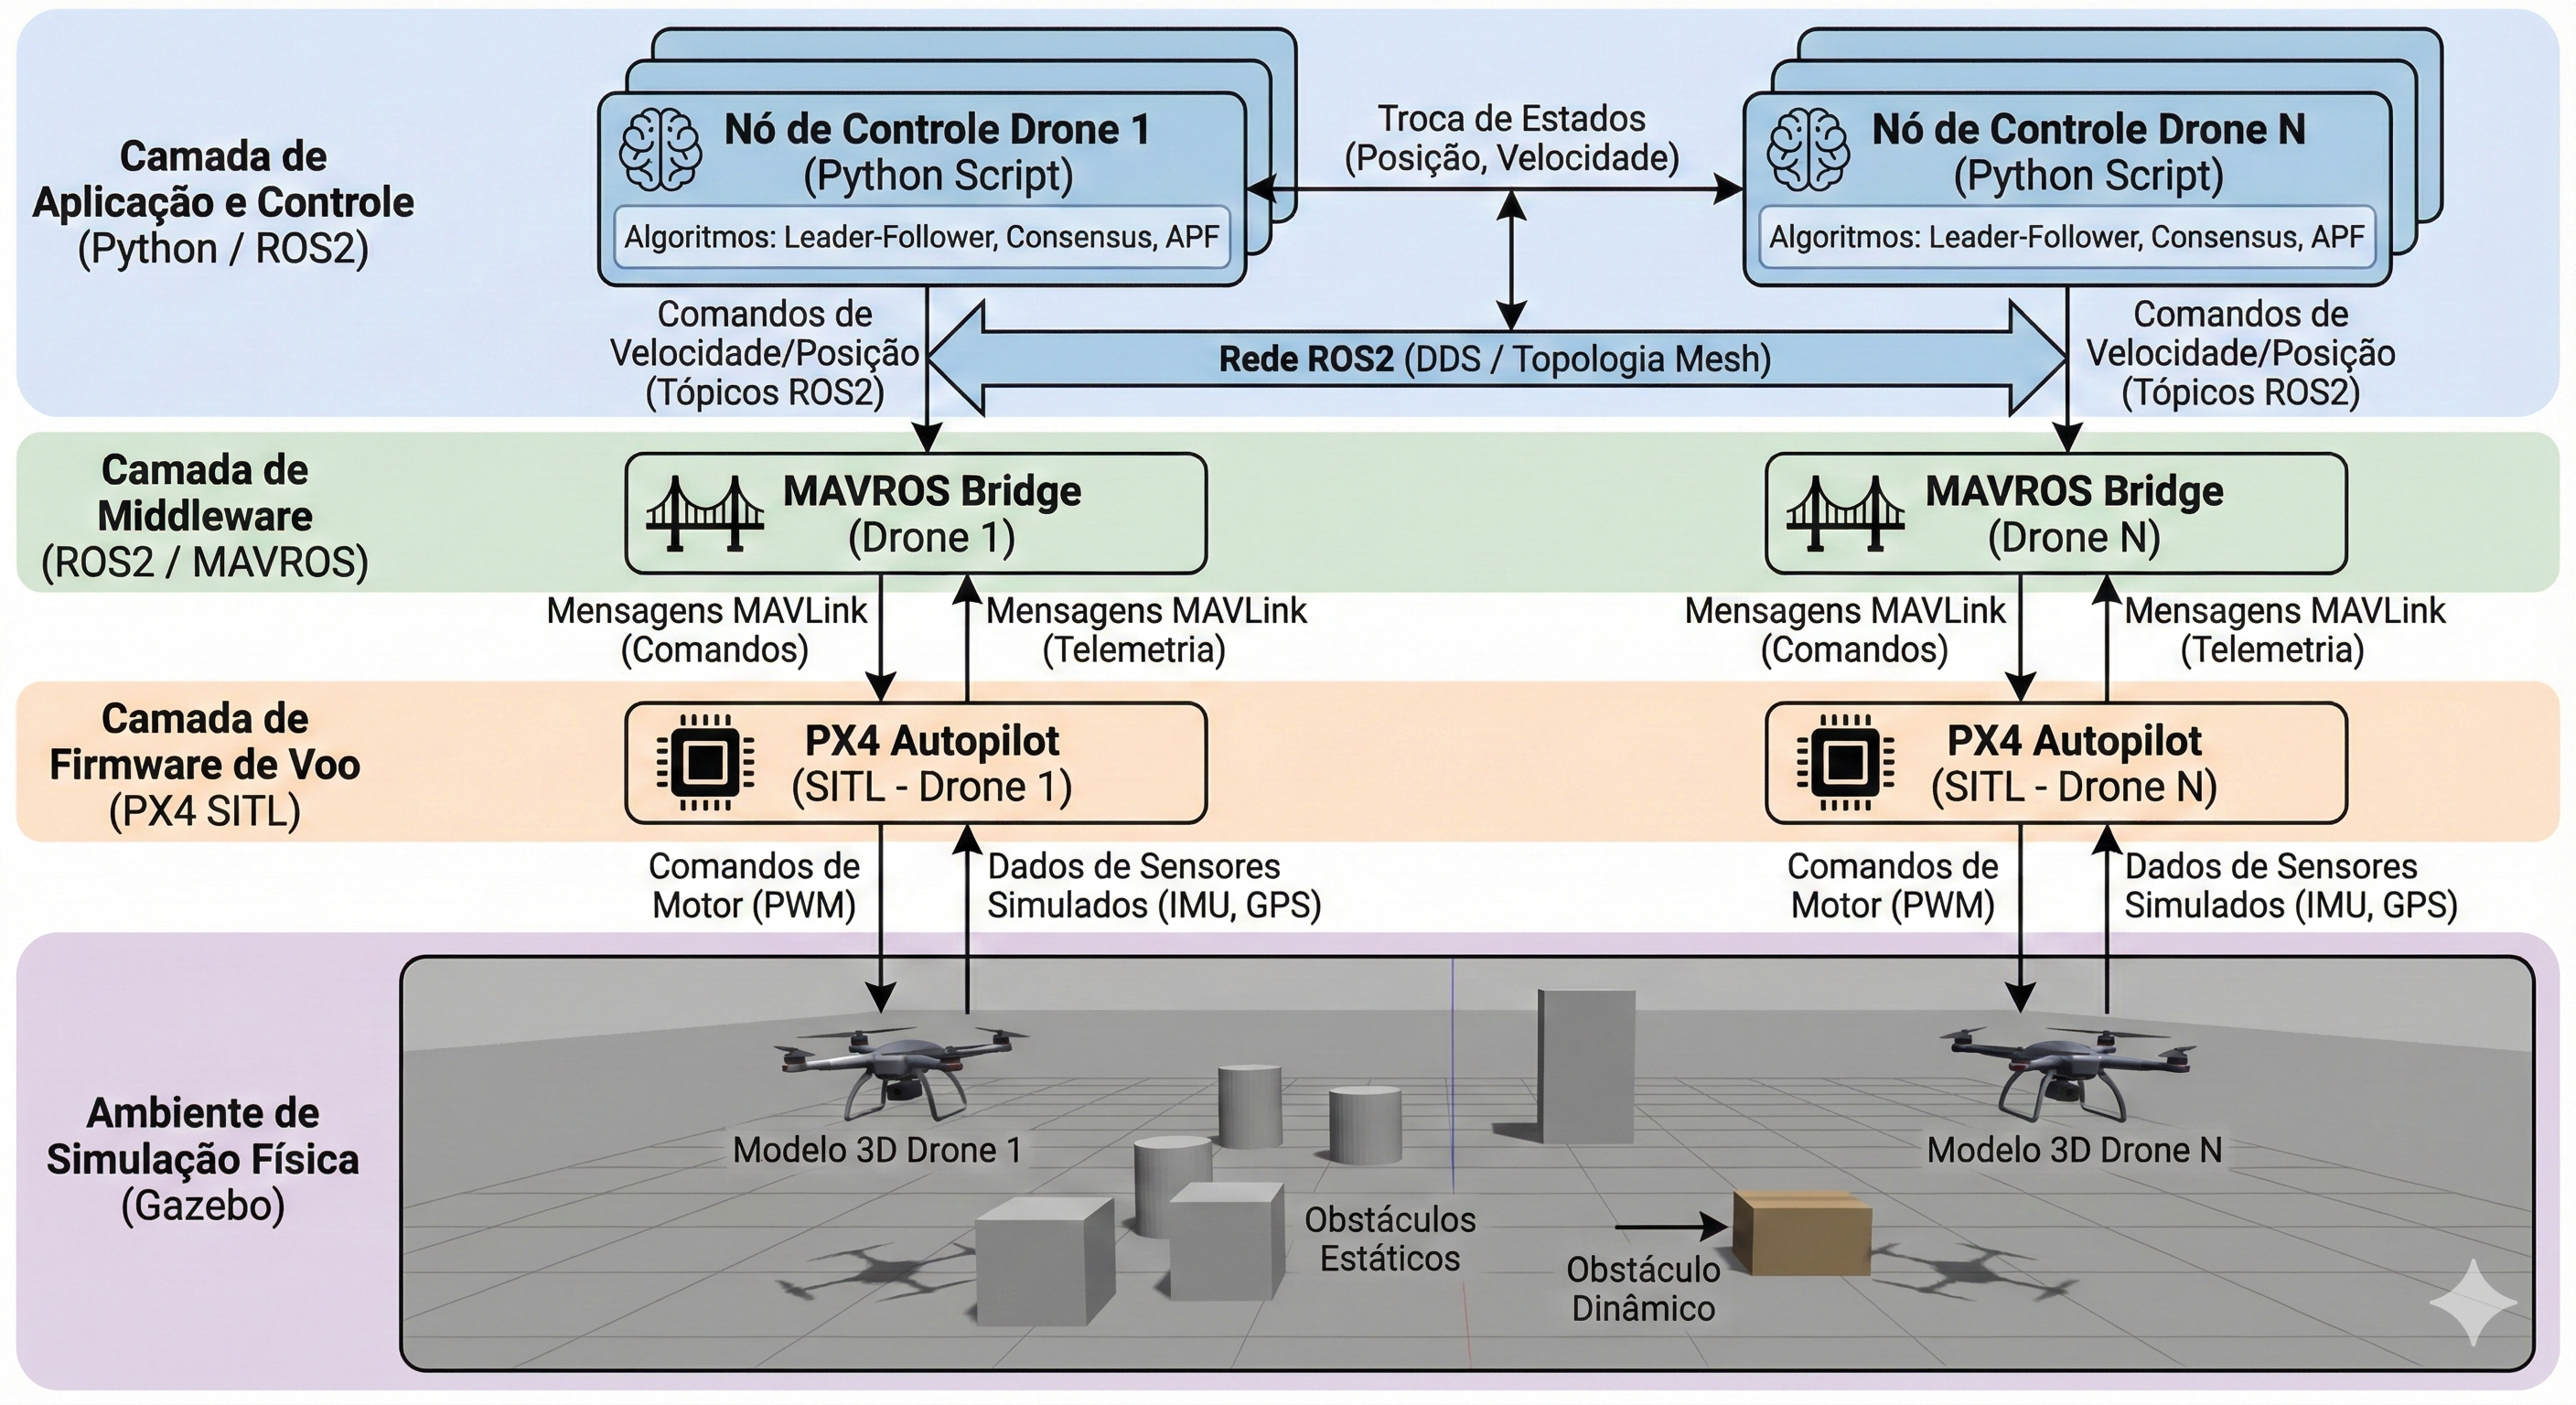
\includegraphics[width=1.0\textwidth]{images/Arquitetura1.png}
    \caption{Arquitetura do sistema de simulação proposto, integrando ROS2, MAVROS, PX4 SITL e Gazebo.}
    \label{fig:Arquitetura de simulação}
\end{figure*}

Visando abranger situações diferentes e assim conseguir avaliar os algoritmos por completo, três cenários experimentais serão configurados:

\begin{enumerate}
    \item \textbf{Espaço Livre}: ambiente sem obstáculos, destinado à análise de formação e manutenção estrutural;
    \item \textbf{Com Obstáculos Estáticos}: inserção de barreiras fixas para avaliar reconfiguração da formação;
    \item \textbf{Com Obstáculos Dinâmicos}: inclusão de obstáculos móveis, permitindo avaliar capacidade de adaptação e resposta.
\end{enumerate}

Para assegurar robustez estatística, cada experimento será repetido 10-20 vezes para cada algoritmo e cada cenário, utilizando condições iniciais distintas geradas por diferentes sementes aleatórias. Esse número de repetições foi definido com base em análise de poder estatístico, garantindo confiabilidade nas comparações entre estratégias. Cada simulação utilizará 4 drones, número suficiente para avaliar o comportamento do algoritmo no cenário.

As métricas utilizadas na avaliação serão inicialmente apenas essas:

\begin{itemize}
    \item \textbf{Erro de Formação (EF)}: distância média entre a posição real e a posição desejada de cada agente;
    \item \textbf{Tempo de Convergência (TC)}: tempo necessário para o sistema estabilizar a formação;
    \item \textbf{Estabilidade e Robustez (ER)}: capacidade de manter a formação diante de falhas de comunicação, distúrbios externos ou eventos inesperados.
\end{itemize}

Essas métricas são suficientes para avaliar a adequação do algoritmo com o cenário experimental avaliado. Os resultados serão analisados de forma quantitativa e gráfica, utilizando curvas de convergência, gráficos de dispersão e estatísticas descritivas como média, variância e desvio padrão. Essa abordagem permite comparar o desempenho das diferentes técnicas de forma detalhada e imparcial, identificando quais algoritmos — ou combinações — apresentam maior eficácia em cada tipo de cenário.

Por fim, o conjunto de procedimentos adotados e a arquitetura de simulação proposta garantem reprodutibilidade, comparabilidade e rigor experimental, permitindo que esta pesquisa contribua de maneira sólida para o avanço do estudo de controle em enxames de VANTs.


